\documentclass[a4paper,11pt,fleqn,twoside,openright]{memoir} 	% Openright aabner kapitler paa hoejresider (openany begge)

%%%% PACKAGES %%%%

% ¤¤ Oversaettelse og tegnsaetning ¤¤ %
%tilføjet af AT
\usepackage{url}
\usepackage{rotating}
\usepackage{pdflscape}

\usepackage[utf8]{inputenc}					% Input-indkodning af tegnsaet (UTF8)
\usepackage[danish]{babel}					% Dokumentets sprog
\usepackage[T1]{fontenc}					% Output-indkodning af tegnsaet (T1)
\usepackage{ragged2e,anyfontsize}			% Justering af elementer
\usepackage{fixltx2e}						% Retter forskellige fejl i LaTeX-kernen	
								\usepackage{blindtext}	
								
% ¤¤ Figurer og tabeller (floats) ¤¤ %
\usepackage{graphicx} 						% Haandtering af eksterne billeder (JPG, PNG, PDF)
\usepackage{multirow}                		% Fletning af raekker og kolonner (\multicolumn og \multirow)
\usepackage{colortbl} 						% Farver i tabeller (fx \columncolor, \rowcolor og \cellcolor)
\usepackage[dvipsnames]{xcolor}				% Definer farver med \definecolor. Se mere: http://en.wikibooks.org/wiki/LaTeX/Colors
\usepackage{flafter}						% Soerger for at floats ikke optraeder i teksten foer deres reference
\let\newfloat\relax 						% Justering mellem float-pakken og memoir
\usepackage{float}							% Muliggoer eksakt placering af floats, f.eks. \begin{figure}[H]
%\usepackage{eso-pic}						% Tilfoej billedekommandoer paa hver side
%\usepackage{wrapfig}						% Indsaettelse af figurer omsvoebt af tekst. \begin{wrapfigure}{Placering}{Stoerrelse}
%\usepackage{multicol}         	        	% Muliggoer tekst i spalter
%\usepackage{rotating}						% Rotation af tekst med \begin{sideways}...\end{sideways}
\usepackage{longtable}

% ¤¤ Matematik mm. ¤¤
\usepackage{amsmath,amssymb,stmaryrd} 		% Avancerede matematik-udvidelser
\usepackage{mathtools}						% Andre matematik- og tegnudvidelser
\usepackage{textcomp}                 		% Symbol-udvidelser (f.eks. promille-tegn med \textperthousand )
\usepackage{siunitx}						% Flot og konsistent praesentation af tal og enheder med \si{enhed} og \SI{tal}{enhed}
\sisetup{output-decimal-marker = {,}}		% Opsaetning af \SI (DE for komma som decimalseparator) 
\usepackage[version=3]{mhchem} 				% Kemi-pakke til flot og let notation af formler, f.eks. \ce{Fe2O3}
%\usepackage{rsphrase}						% Kemi-pakke til RS-saetninger, f.eks. \rsphrase{R1}

% ¤¤ Referencer og kilder ¤¤ %
\usepackage[danish]{varioref}				% Muliggoer bl.a. krydshenvisninger med sidetal (\vref)
\usepackage{natbib}							% Udvidelse med naturvidenskabelige citationsmodeller
%\usepackage{xr}							% Referencer til eksternt dokument med \externaldocument{<NAVN>}
%\usepackage{glossaries}					% Terminologi- eller symbolliste (se mere i Daleifs Latex-bog)

% ¤¤ Misc. ¤¤ %
\usepackage{listings}						% Placer kildekode i dokumentet med \begin{lstlisting}...\end{lstlisting}
\usepackage{lipsum}							% Dummy text \lipsum[..]
\usepackage[shortlabels]{enumitem}			% Muliggoer enkelt konfiguration af lister
\usepackage{pdfpages}						% Goer det muligt at inkludere pdf-dokumenter med kommandoen \includepdf[pages={x-y}]{fil.pdf}	
\pdfoptionpdfminorversion=6					% Muliggoer inkludering af pdf dokumenter, af version 1.6 og hoejere
\pretolerance=2500 							% Justering af afstand mellem ord (hoejt tal, mindre orddeling og mere luft mellem ord)

% Kommentarer og rettelser med \fxnote. Med 'final' i stedet for 'draft' udloeser hver note en error i den faerdige rapport.
\usepackage[footnote,draft,danish,silent,nomargin]{fixme}		


%%%% CUSTOM SETTINGS %%%%

% ¤¤ Marginer ¤¤ %
\setlrmarginsandblock{3.5cm}{2.5cm}{*}		% \setlrmarginsandblock{Indbinding}{Kant}{Ratio}
\setulmarginsandblock{2.5cm}{3.0cm}{*}		% \setulmarginsandblock{Top}{Bund}{Ratio}
\checkandfixthelayout 						% Oversaetter vaerdier til brug for andre pakker

%	¤¤ Afsnitsformatering ¤¤ %
\setlength{\parindent}{0mm}           		% Stoerrelse af indryk
\setlength{\parskip}{3mm}          			% Afstand mellem afsnit ved brug af double Enter
\linespread{1,1}							% Linie afstand

% ¤¤ Litteraturlisten ¤¤ %
\bibpunct[,]{[}{]}{;}{a}{,}{,} 				% Definerer de 6 parametre ved Harvard henvisning (bl.a. parantestype og seperatortegn)
\bibliographystyle{bibtex/harvard}			% Udseende af litteraturlisten.

% ¤¤ Indholdsfortegnelse ¤¤ %
\setcounter{secnumdepth}{4}		 			% Dybden af nummerede overkrifter (part/chapter/section/subsection)
\setcounter{maxsecnumdepth}{4}					% Dokumentklassens graense for nummereringsdybde
\setcounter{tocdepth}{4} 					% Dybden af indholdsfortegnelsen

% ¤¤ Lister ¤¤ %
\setlist{
  topsep=0pt,								% Vertikal afstand mellem tekst og listen
  itemsep=-1ex,								% Vertikal afstand mellem items
} 

% ¤¤ Visuelle referencer ¤¤ %
\usepackage[colorlinks]{hyperref}			% Danner klikbare referencer (hyperlinks) i dokumentet.
\hypersetup{colorlinks = true,				% Opsaetning af farvede hyperlinks (interne links, citeringer og URL)
    linkcolor = black,
    citecolor = black,
    urlcolor = black
}

% ¤¤ Opsaetning af figur- og tabeltekst ¤¤ %
\captionnamefont{\small\bfseries\itshape}	% Opsaetning af tekstdelen ('Figur' eller 'Tabel')
\captiontitlefont{\small}					% Opsaetning af nummerering
\captiondelim{. }							% Seperator mellem nummerering og figurtekst
\hangcaption								% Venstrejusterer flere-liniers figurtekst under hinanden
\captionwidth{\linewidth}					% Bredden af figurteksten
\setlength{\belowcaptionskip}{0pt}			% Afstand under figurteksten
		
% ¤¤ Opsaetning af listings ¤¤ %
\definecolor{commentGreen}{RGB}{34,139,24}
\definecolor{stringPurple}{RGB}{208,76,239}

\lstset{language=Matlab,					% Sprog
	basicstyle=\ttfamily\scriptsize,		% Opsaetning af teksten
	keywords={for,if,while,else,elseif,		% Noegleord at fremhaeve
			  end,break,return,case,
			  switch,function},
	keywordstyle=\color{blue},				% Opsaetning af noegleord
	commentstyle=\color{commentGreen},		% Opsaetning af kommentarer
	stringstyle=\color{stringPurple},		% Opsaetning af strenge
	showstringspaces=false,					% Mellemrum i strenge enten vist eller blanke
	numbers=left, numberstyle=\tiny,		% Linjenumre
	extendedchars=true, 					% Tillader specielle karakterer
	columns=flexible,						% Kolonnejustering
	breaklines, breakatwhitespace=true,		% Bryd lange linjer
}

% ¤¤ Navngivning ¤¤ %
\addto\captionsdanish{
	\renewcommand\appendixname{Appendiks}
	\renewcommand\contentsname{Indholdsfortegnelse}	
	\renewcommand\appendixpagename{Appendiks}
	\renewcommand\appendixtocname{Appendiks}
	\renewcommand\cftchaptername{\chaptername~}				% Skriver "Kapitel" foran kapitlerne i indholdsfortegnelsen
	\renewcommand\cftappendixname{\appendixname~}			% Skriver "Appendiks" foran appendiks i indholdsfortegnelsen
}

% ¤¤ Kapiteludssende ¤¤ %
\definecolor{numbercolor}{gray}{0.7}		% Definerer en farve til brug til kapiteludseende
\newif\ifchapternonum

\makechapterstyle{jenor}{					% Definerer kapiteludseende frem til ...
  \renewcommand\beforechapskip{0pt}
  \renewcommand\printchaptername{}
  \renewcommand\printchapternum{}
  \renewcommand\printchapternonum{\chapternonumtrue}
  \renewcommand\chaptitlefont{\fontfamily{pbk}\fontseries{db}\fontshape{n}\fontsize{25}{35}\selectfont\raggedleft}
  \renewcommand\chapnumfont{\fontfamily{pbk}\fontseries{m}\fontshape{n}\fontsize{1in}{0in}\selectfont\color{numbercolor}}
  \renewcommand\printchaptertitle[1]{%
    \noindent
    \ifchapternonum
    \begin{tabularx}{\textwidth}{X}
    {\let\\\newline\chaptitlefont ##1\par} 
    \end{tabularx}
    \par\vskip-2.5mm\hrule
    \else
    \begin{tabularx}{\textwidth}{Xl}
    {\parbox[b]{\linewidth}{\chaptitlefont ##1}} & \raisebox{-15pt}{\chapnumfont \thechapter}
    \end{tabularx}
    \par\vskip2mm\hrule
    \fi
  }
}											% ... her

\chapterstyle{jenor}						% Valg af kapiteludseende - Google 'memoir chapter styles' for alternativer

% ¤¤ Sidehoved ¤¤ %

\makepagestyle{Uni}							% Definerer sidehoved og sidefod udseende frem til ...
\makepsmarks{Uni}{%
	\createmark{chapter}{left}{shownumber}{}{. \ }
	\createmark{section}{right}{shownumber}{}{. \ }
	\createplainmark{toc}{both}{\contentsname}
	\createplainmark{lof}{both}{\listfigurename}
	\createplainmark{lot}{both}{\listtablename}
	\createplainmark{bib}{both}{\bibname}
	\createplainmark{index}{both}{\indexname}
	\createplainmark{glossary}{both}{\glossaryname}
}
\nouppercaseheads											% Ingen Caps oenskes

\makeevenhead{Uni}{Langerhanske Øer}{}{\leftmark}				% Definerer lige siders sidehoved (\makeevenhead{Navn}{Venstre}{Center}{Hoejre})
\makeoddhead{Uni}{\rightmark}{}{Ingeniørhøjskolen Aarhus}			% Definerer ulige siders sidehoved (\makeoddhead{Navn}{Venstre}{Center}{Hoejre})
\makeevenfoot{Uni}{\thepage}{}{}							% Definerer lige siders sidefod (\makeevenfoot{Navn}{Venstre}{Center}{Hoejre})
\makeoddfoot{Uni}{}{}{\thepage}								% Definerer ulige siders sidefod (\makeoddfoot{Navn}{Venstre}{Center}{Hoejre})
\makeheadrule{Uni}{\textwidth}{0.5pt}						% Tilfoejer en streg under sidehovedets indhold
\makefootrule{Uni}{\textwidth}{0.5pt}{1mm}					% Tilfoejer en streg under sidefodens indhold

\copypagestyle{Unichap}{Uni}								% Sidehoved for kapitelsider defineres som standardsider, men med blank sidehoved
\makeoddhead{Unichap}{}{}{}
\makeevenhead{Unichap}{}{}{}
\makeheadrule{Unichap}{\textwidth}{0pt}
\aliaspagestyle{chapter}{Unichap}							% Den ny style vaelges til at gaelde for chapters
															% ... her
															
\pagestyle{Uni}												% Valg af sidehoved og sidefod (benyt "plain" for ingen sidehoved/fod)


%%%% CUSTOM COMMANDS %%%%

% ¤¤ Billede hack ¤¤ %										% Indsaet figurer nemt med \figur{Stoerrelse}{Fil}{Figurtekst}{Label}
\newcommand{\figur}[4]{
		\begin{figure}[H] \centering
			\includegraphics[width=#1\textwidth]{billeder/#2}
			\caption{#3}\label{#4}
		\end{figure} 
}

% ¤¤ Specielle tegn ¤¤ %
\newcommand{\decC}{^{\circ}\text{C}}
\newcommand{\dec}{^{\circ}}
\newcommand{\m}{\cdot}


%%%% ORDDELING %%%%

\hyphenation{}											% Preamble indlaeses
\raggedbottom													% Soerger for at LaTeX ikke "straekker" teksten

%\includeonly{file1,file2}										% Inkluder kun specifikke filer (kommasepareret liste)

\begin{document}												% Starter dokumentet - obligatorisk


\frontmatter													% Forindhold - nummereres med romertal

\thispagestyle{empty}
\begin{center}
\vspace{3cm}

\phantom{hul}

\phantom{hul}

\phantom{hul}

\textsl{\LARGE Cell sorter for isolation of insulin producing cells} \\ \vspace{0.25cm}
\textsl{\Large Projektdokumentation} \\ %\vspace{1cm}

\rule{13cm}{3mm} \\ \vspace{1cm}

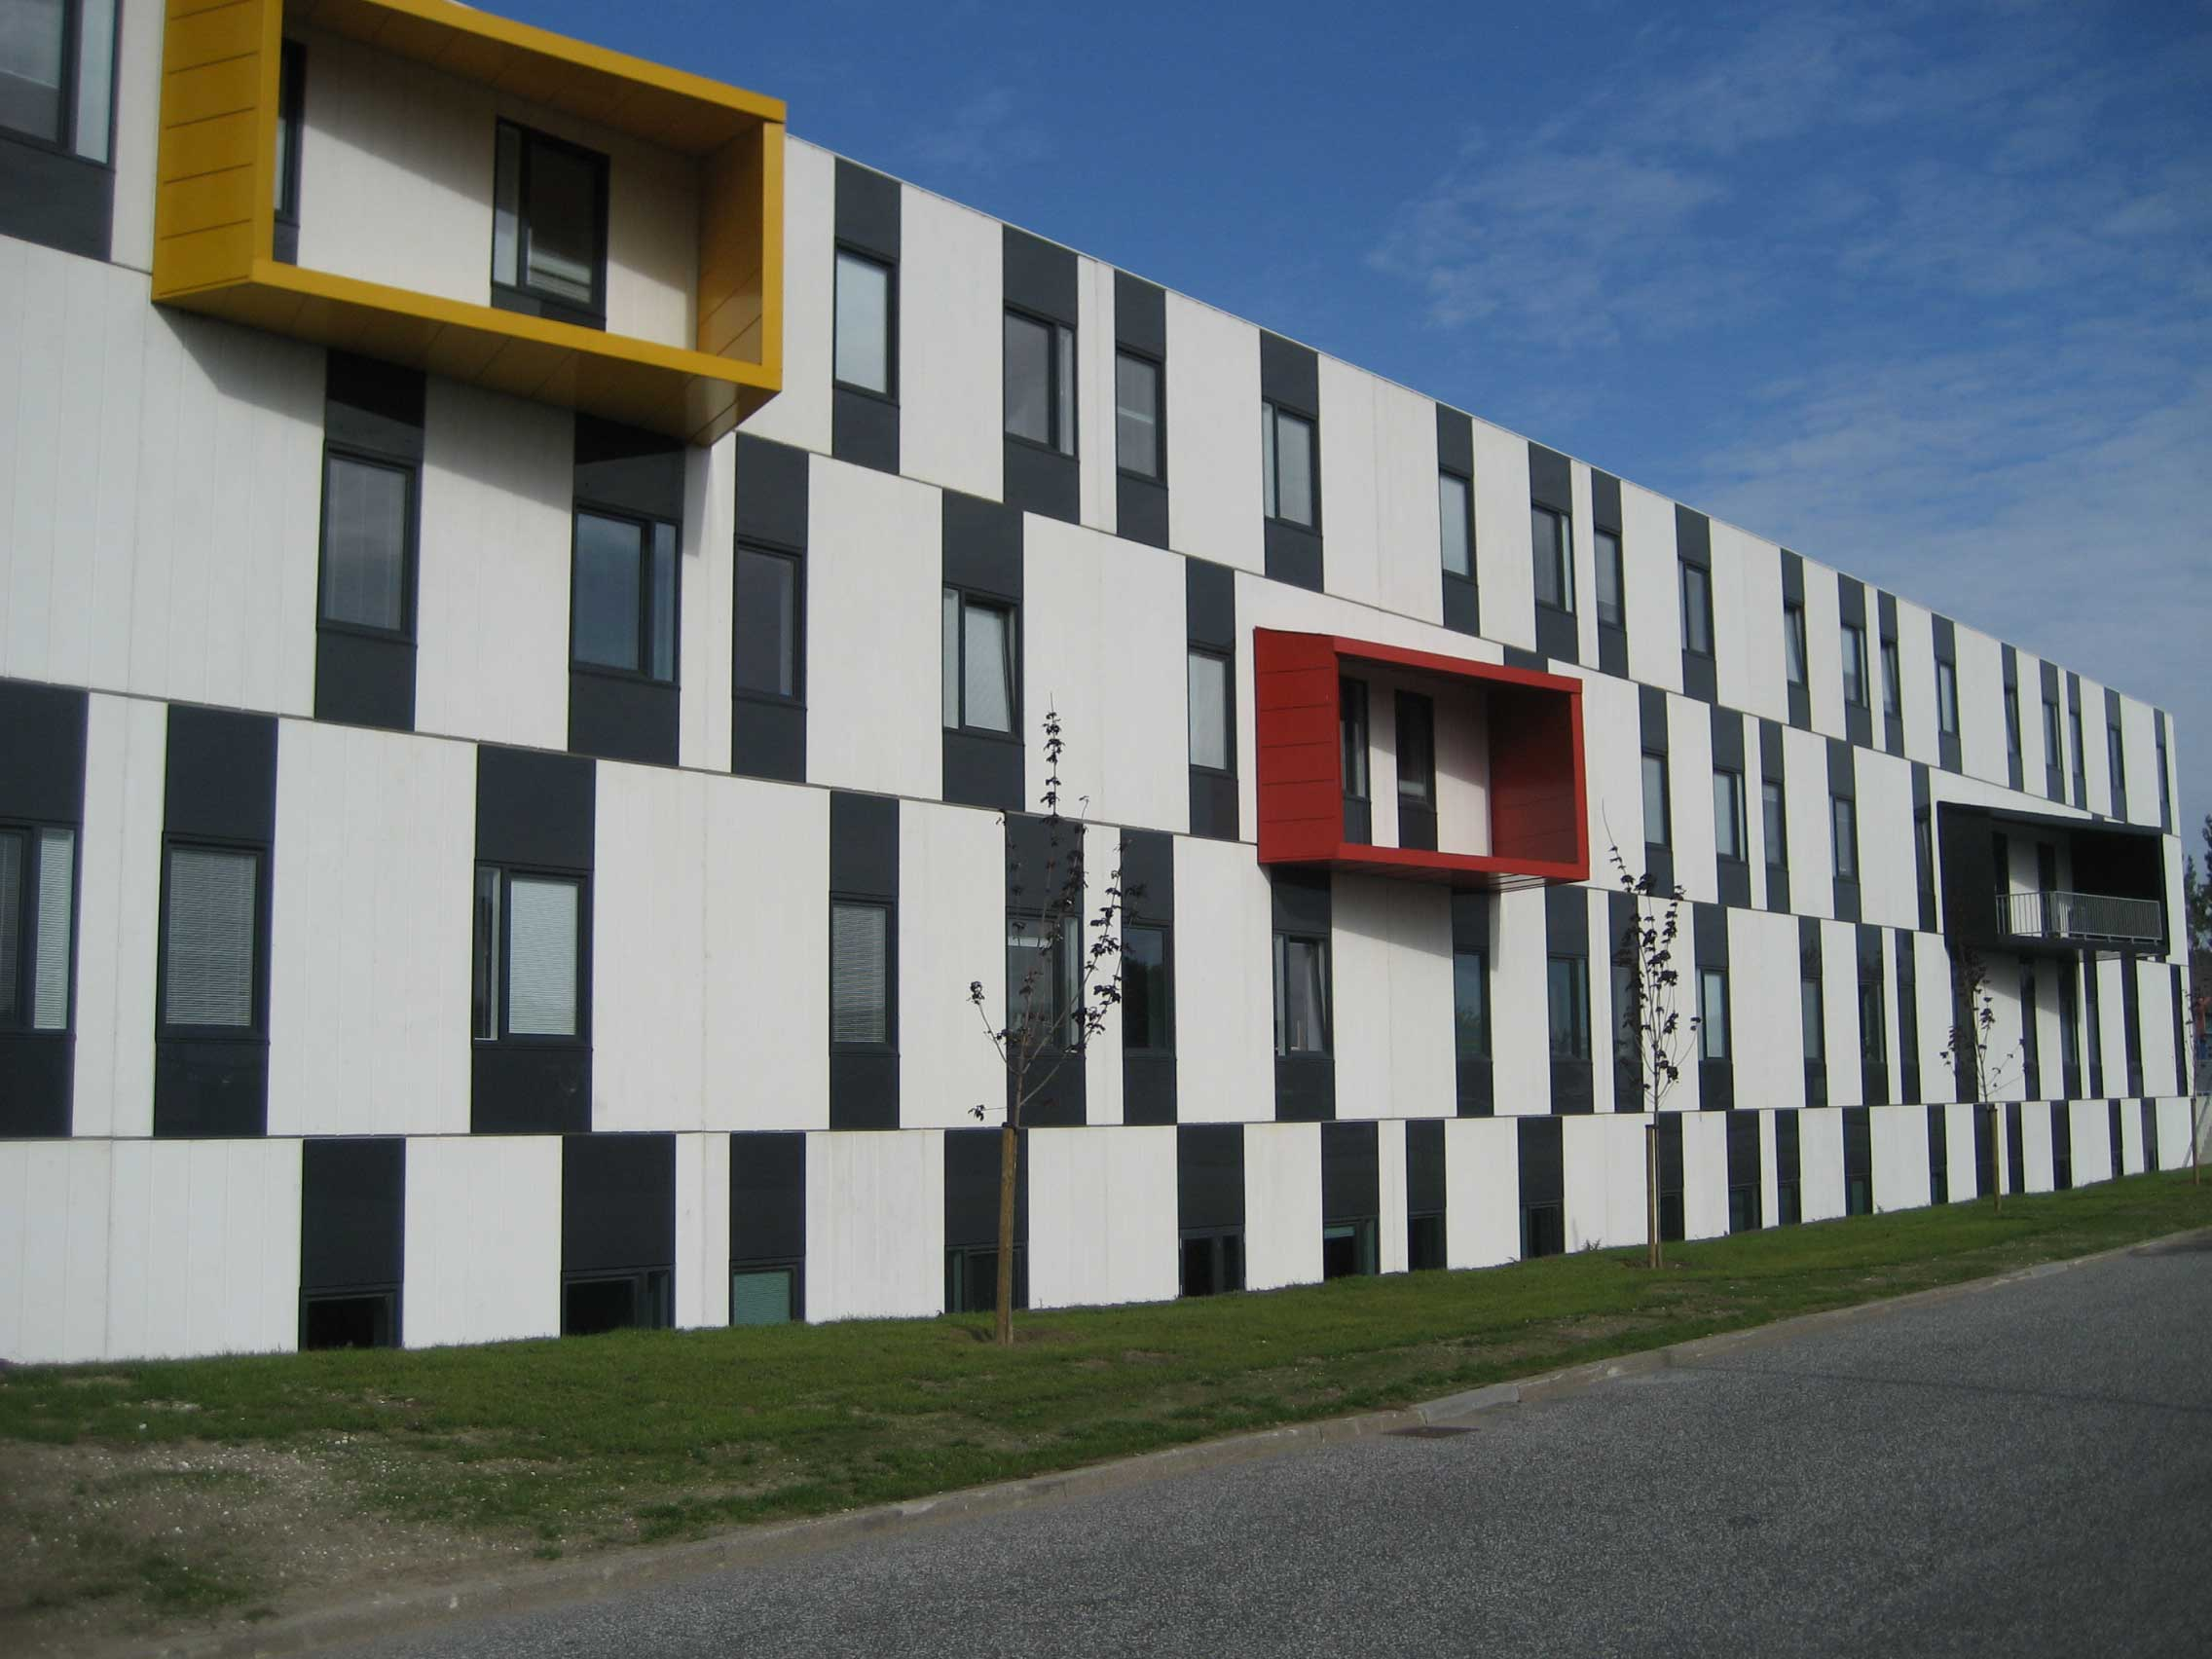
\includegraphics[width=0.9\textwidth]{billeder/forside.jpg}

\textsc{\center Bachelorprojekt \\
Projektnr: 15137 \\
Ingeniørhøjskolen, Aarhus Universitet \\
Den 16. december 2015 \\ \vspace{1cm}
11242	Anders Toft Andersen \\
201270874	Anders Esager \\
Projektvejleder: Samuel Alberg Thrysøe \\}
\end{center}

\cleardoublepage												% Indsaetter tom side, saa naeste kapitel starter paa hoejre side (hvis noedvendigt)
% Dette er et titelblad designet til videregående uddannelser på et universitet
% Filen kræver:
% Universitetets logo:  AU-logo-DK eller AU-logo-DK
% Synopsis: En fil ved navn synopsis.tex

% Udarbejdet af: Jesper Nørgaard (jesper@noergaard.eu) 10. april 2012

\phantomsection
\pdfbookmark[0]{Titelblad}{titelblad}
\thispagestyle{empty}

\begin{minipage}[t]{0.48\textwidth}
\vspace*{-8pt}			

\includegraphics[height=2.5cm]{billeder/AU-logo-DK}
\end{minipage}
\hfill
\begin{minipage}[t]{0.48\textwidth}
{\small 
\textbf{Studienævn for Aarhus School of Science}\\
Nordre Ringgade 1 \\
8000 Aarhus C \\
Tlf: 8715 0000 \\
http://www.au.dk}
\end{minipage}

\vspace*{1cm}

\begin{minipage}[t]{0.48\textwidth}
\textbf{Titel:} \\[5pt]\bigskip\hspace{2ex}
Energirenovering

\textbf{Projekt:} \\[5pt]\bigskip\hspace{2ex}
P1-projekt

\textbf{Projektperiode:} \\[5pt]\bigskip\hspace{2ex}
September 2014 - December 2014

\textbf{Projektgruppe:} \\[5pt]\bigskip\hspace{2ex}
B131	

\textbf{Deltagere:} \\[5pt]\hspace*{2ex}
Adam  G. Hansen \\\hspace*{2ex}
Berit Jørgensen \\\hspace*{2ex}
Christoffer Haning \\\hspace*{2ex}
Dorthe Møller \\\hspace*{2ex}
Ejnar V. Jensen \\\hspace*{2ex}
Freja Poulsen \\\bigskip\hspace{2ex}
Gerhard Pedersen

\textbf{Vejledere:} \\[5pt]\hspace*{2ex}
Carsten Henningsen \\\bigskip\hspace{2ex}
Lotte Dalgaard

\vspace*{1cm}

\textbf{Oplagstal: 10} \\
\textbf{Sidetal: 80} \\
\textbf{Appendiks: 3} \\ 
\textbf{Afsluttet 18-12-2014}

\end{minipage}
\hfill
\begin{minipage}[t]{0.483\textwidth}
Synopsis: \\[5pt]
\fbox{\parbox{7cm}{\bigskipSynopsis

\bigskip}}
\end{minipage}

\vfill

{\footnotesize\itshape Rapportens indhold er frit tilgængeligt, men offentliggørelse (med kildeangivelse) må kun ske efter aftale med forfatterne.}

% Rapportens indhold er frit tilgængeligt, men offentliggørelse (med kildeangivelse) må kun ske efter aftale med forfatterne.
% The content of the report is freely available, but publication (with source reference) may only take place in agreement with the authors.

\cleardoublepage
\chapter*{Forord}

Denne rapport er udarbejdet som en del af syvende semesters bachelorprojekt på Ingeniørhøjskolen, Aarhus Universitet. Rapporten er udarbejdet af en projektgruppe bestående af 2 sundhedsteknologistuderende. Projektet er udarbejdet i samarbejde med Søren Gregersen, overlæge på Medicinsk Endokrinologisk Afdeling på Aarhus Universitetshospital med hjælp fra Per. B. Jeppesen, Lektor ved Institut for Klinisk Medicin, Aarhus Universitet. Bachelorprojektet er udført i perioden 28. august 2015 til 16. december 2015, hvor forprojektet er udført i perioden 26. april 2015 til 15. juni 2015.  

Projektgruppen retter en stor tak til Søren Gregersen for samarbejdet, ligeledes skal der gives en tak til Per B. Jeppesen. Ydermere skal der lyde en varm tak til gruppens vejleder Samuel Thrysøe, der har hjulpet og støttet gruppen igennem hele processen. Endelig skal der gives en tak til reviewgruppen bestående af Simon Vammen Grønbæk og Karl-John Schmidt, som har bestået med konstruktiv kritik og rettelser. 


%Dette dokument indeholder projektdokumentationen for projektet \textit{Cell sorter for isolation of insulin producing cells}. Dokumentet indeholder kravspecifikation og accepttest for systemet, samt beskrivelse af projektets design og implementeringsfase. 

%Kravspecifikationen er udarbejdet i samarbejde med Søren Gregersen, overlæge på Medicinsk Endokrinologisk Afdeling, Aarhus Universitetshospital, der agerer som projektets kunde. 



\phantom{Luft}

\phantom{Luft}

\begin{table}[H]
	\centering
		\begin{tabular}{c c}
			\underline{\phantom{mmmmmmmmmmmmmm}} & \underline{\phantom{mmmmmmmmmmmmmm}}  \\
			Anders Toft Andersen			& Anders Esager		 			\\ 										\end{tabular}
\end{table}

\section*{Læsevejledning}
Rapporten indeholder primært metoder, resultater og diskussioner til produktet, som gruppen har udarbejdet. Der vil igennem rapporten fremtræde kildehenvisninger, og disse vil være samlet i en kildeliste bagerst i rapporten. Der er i rapporten anvendt kildehenvisning efter Harvardmetoden, i teksten refereres en kilde med [Efternavn, År]. Denne henvisning fører til kildelisten, hvor bøger er angivet med forfatter, titel, udgave og forlag, mens internetsider er angivet med forfatter, titel og dato. Til sidst i rapporten er bilagsliste, som anskueliggør filnavnene i den afleverede bilagsmappen. Diagrammerne udarbejdet i projektet er skrevet på engelsk. 

I bilagslisten forefindes alle filerne, der er afleveret ved siden af rapporten, herunder datablade, Matlab-kode, Eagle kilde-filer og Gerber-filer. Herudover er den udfyldte accepttest og fejlrapport vedlagt som bilag.

Ved siden af rapporten er vedlagt en video, som viser den udviklede prototype.

%Der vil igennem rapporten fremtræde kildehenvisninger, og disse vil være samlet i en kildeliste bagerst i rapporten. Der er i rapporten anvendt kildehenvisning efter Harvardmetoden, så i teksten refereres en kilde med [Efternavn, År]. Denne henvisning fører til kildelisten, hvor bøger er angivet med forfatter, titel, udgave og forlag, mens Internetsider er angivet med forfatter, titel og dato. Figurer og tabeller er nummereret i henhold til kapitel, dvs. den første figur i kapitel 7 har nummer 7.1, den anden, nummer 7.2 osv. Forklarende tekst til figurer og tabeller findes under de givne figurer og tabeller.

\cleardoublepage

%%%% Indholdsfortegnelse (TOC) %%%%

\phantomsection													% Kunstigt afsnit, som hyperlinks kan 'holde fast i'
\pdfbookmark[0]{Indholdsfortegnelse}{indhold}					% Tildeler en klikbar bookmark til den endelige PDF
\tableofcontents*												% Indholdsfortegnelsen (kaldet ToC) 

%\addtocontents{toc}{\protect\newpage}							% Fremtvinger sideskift i ToC hvis noedvendig (der hvor koden placeres)


\mainmatter														% Hovedindhold - nummereres fra side 1

%%%% Rapportindhold %%%% 										% Rapportindholdet boer IKKE indeholde broedtekst - KUN includede filer!

%% Indledende %%												% Opdel evt. i passende afsnit for overblikkets skyld

\section{Indledning}
Dette dokument indeholder accepttesten for the Cell Collector(omtales herefter som systemet). 

\subsection{Formål}
Formålet med dokumentet er at sikre at alle krav til produktet er opfyldt, i henhold til kravspecifikationen.

\chapter{Projektbeskrivelse}

Projektforslaget lægger op til at belyse effekterne af energirenovering samt hvordan barrierne overvindes ved brug af virkemidler. 

I det følgende reflekteres der over emnerne i problemanalysen. Problemformuleringen indrammer herefter projektet inden det konkretiseres i afgrænsningen. Endelig beskrives de metoder, som søges anvendt. 

\section{Problemanalyse}

\section{Problemformulering}

I den kontekstuelle del søges følgende spørgsmål besvaret.

I den tekniske del søges følgende energi- og konstruktionsmæssige spørgsmål besvaret.

\section{Projektafgrænsning}

\section{Metode}
\chapter{Kravspecifikation}

\section{Indledning}
Dette dokument indeholder kravspecifikationen for The Cell Collector(omtales herefter som systemet). Dokumentet er udarbejdet i samarbejde med kunden(Søren Gregersen) og specificerer kundens kvalitetskrav, samt funktionelle og ikke funktionelle krav. Der er sammen med kunden udarbejdet en accepttest, som har til formål at teste de specificerede krav i kravspecifikation.
\section{Versionshistorik}
Tabel...

\section{Systembeskrivelse}
Formålet med projektet er at udvikle et system til isolation af insulin producerende celler (Langerhanske Øer). Mange farmaceutiske virksomheder og forskningsafdelinger udfører forsøg på disse øer fra bl.a. rotter. Processen med isolering af Langerhanske øer startes ved operativt at fjerne pancreas, hvorefter vævet opløses vha. enzymet kollagenase. Når vævet er opløst fortyndes det yderligere inden det hældes i petriskåle. Øerne bliver herefter manuelt isoleret vha. mikroskop og diverse præcisions redskaber. Denne proces er både besværlig og tidskrævende. Formålet med projektet er derfor, at udvikle en ny metode til isolation af cellerne. Systemet skal indeholder en beholder til opløsningen med langerhanske øer. Denne opløsning skal føres ud gennem en tynd slange(<0,5mm)  forbi et kamera, hvor der ved hjælp af Matlab skal udføres billedprocessering. Billedebehandlingen skal genkende, hvornår der er en langerhanske ø. Derefter skal systemet frasortere denne, ved et ventil system der åbner på det rigtige tidspunkt. Til at skabe flowet i slangerne anvendes en pumpe.  Et krav til pumpen er at den skal være nænsom ved celleopløsningen, da de langerhanske øer er meget skrøbelige.
En automatiseret løsning af sorteringsprocessen kan bidrage med reducering af omkostningerne, give en mere ensartet sortering samt sikre dokumentation af de sorterede øer. Systemet kan fra et kommercielt synspunkt bidrage til basal forskning og til screening af nye medicinske præparater.

Indsæt figur!!
\section{Funktionelle krav}
\subsection{Aktør beskrivelse}
Systemets primære aktør er operatøren, som står for påfyldning af celler, start og stop af sorteringsprocessen. Operatøren har mulighed for at interagere med systemet via en grafisk brugergrænseflade. Systemets sekundære aktør er PC’ens filsystem, hvor der løbende gemmes en log over sorteringsprocessen.
\subsection{Use Case Diagram}
Indsæt figur!!
%\subsection{Use Case 1 - Start sorteringscyklus}
\label{uc:1}
\begin{center}
		\begin{longtable}{ | m{4cm} | m{8cm}| } 
			\hline
			Mål & Start sorteringscyklus \\ 
			\hline
			Initiering &  Use casen initieres af operatøren\\
			\hline
			Aktør & 
			Primær: Operatør
			
			 Sekundær: Kamera			  \\ 
			\hline
			Startbetingelser & The Cell Collector programmet er startet på computeren \\ 
			\hline	
			Slutbetingelser ved succes & Systemet starter med sorteringen af Langerhanske øer \\
			\hline
			Slutbetingelser ved undtagelse & N/A \\
			\hline
			Normalforløb & \begin{enumerate}
				%\setlength\itemsep{0cm} % Decrease line distance
				\item Operatør fylder celleopløsningsbeholderen
				\item Celleopløsningsbeholderen er fyldt
				\item Operatør starter sorteringscyklus ved at klikke på [Start]
				\subitem [Undtagelse 1: Wastebeholder er fyldt] 
				\item Systemet initialiserer Arduinoen
				\subitem [Undtagelse 2: Ingen forbindelse til Arduino]
				\item Systemet kontrollerer celleopløsningsbeholderen ved at konvertere spændingen (\SI{}{\volt})  til \SI{}{\milli\litre}, og vise beholderens indhold (\SI{}{\milli\litre}) på GUI
				\item Systemet initialiserer kameraet
				\subitem [Undtagelse 3: Kameraet initialiserer ikke]
				\item Systemet tænder for kamera lyset
				\item Systemet tænder for pumpen
				
			\end{enumerate} \\ 
			\hline
			Undtagelser & [Undtagelse 1: Wastebeholder er fyldt] 
			
			\begin{enumerate}
			\item Systembesked: Tøm venligst Wastebeholder før start
			\item Operatøren trykker “OK”
			\item Systemet fortsætter opstartprocessen
			\end{enumerate} 
			
			[Undtagelse 2: Ingen forbindelse til Arduino]
			
			\begin{enumerate}
			\item 1.	Systembesked: Ingen forbindelse til Arduino, kontrollér forbindelser.
			\end{enumerate} 
	
			[Undtagelse 3: Kameraet initialiseres ikke]
			
			\begin{enumerate}
			\item System fejlmeddelse: Kameraet er ikke initialiseret:
			\item Genstart initialisering af Kameraet
			\end{enumerate} \\
			\hline
		\end{longtable}
		
	\end{center}
	\pagebreak
\subsection{Use case 2 - Sortering af Langerhanske Øer}
\label{uc:2}
\begin{center}
		\begin{longtable}{ | m{4cm} | m{8cm}| } 
			\hline
			Mål & Sortere Langerhanske Øer \\ 
			\hline
			Initiering &  Use casen initieres af [UC 1: Startsorteringscyklus]\\
			\hline
			Aktør & Kamera \\ 
			\hline
			Startbetingelser & Systemet er startet og sorteringscyklussen er i gang\\ 
			\hline	
			Slutbetingelser ved succes & Systemet har isoleret en Langerhansk ø og ventilen er lukket \\
			\hline
			Slutbetingelser ved undtagelse & \\
			\hline
			Normalforløb & \begin{enumerate}
				%\setlength\itemsep{0cm} % Decrease line distance
				\item Systemet detekterer en Langerhansk ø
				\item Arduino sender signal til ventilen om åbning
				\item Ventilen åbner
				\item Arduino sender signal til ventilen om lukning
				\item Ventilen lukker
			\end{enumerate} \\ 
			\hline
			Undtagelser & \\
			\hline
		\end{longtable}
		
	\end{center}
	\pagebreak
\subsection{Use Case 3 - Stop sorteringscyklus}
\begin{center}
		\begin{longtable}{ | m{4cm} | m{8cm}| } 
			\hline
			Mål & Stop sorteringscyklus \\ 
			\hline
			Initiering &  Use casen initieres af operatøren\\
			\hline
			Aktør & Operatør \\ 
			\hline
			Startbetingelser & [UC 2: Sortering af Langerhanske Øer] er startet\\ 
			\hline	
			Slutbetingelser ved succes & [UC 2: Sortering af Langerhanske Øer] er stoppet \\
			\hline
			Slutbetingelser ved undtagelse & N/A \\
			\hline
			Normalforløb & \begin{enumerate}
				\setlength\itemsep{0cm} % Decrease line distance
				\item Operatør stopper sorteringscyklussen ved at trykke på [Stop]
				\subitem [Undtagelse 1: Tom celleopløsningsbeholder]
				\item Systemet slukker for pumpen
				\item Systemet slukker for kameraet
				\item Systemet slukker for kamera lyset
				\item Systemet slukker for Arduino
			\end{enumerate} \\ 
			\hline
			Undtagelser & TODO!!\\
			\hline
		\end{longtable}
		
	\end{center}
	\pagebreak
\subsection{Use case 4 - Indstillinger}
\begin{center}
		\begin{longtable}{ | m{4cm} | m{8cm}| } 
			\hline
			Mål & Ændre systemets indstillinger \\ 
			\hline
			Initiering &  Use casen initieres af operatør\\
			\hline
			Aktør & Operatør \\ 
			\hline
			Startbetingelser & [UC 2: Sortering af Langerhanske Øer] er endnu ikke startet\\ 
			\hline	
			Slutbetingelser ved succes & Systemets indstillinger er ændret \\
			\hline
			Slutbetingelser ved undtagelse & Systemets indstillinger er uændret \\
			\hline
			Normalforløb & \begin{enumerate}
				%\setlength\itemsep{0cm} % Decrease line distance
				\item Operatøren klikker på [Indstillinger]
				\item Et nyt vindue åbner med systemets indstillinger.
				\item Operatøren vælger de ønskede indstillinger, og trykker [Gem indstillinger]
				\subitem [Undtagelse 1: Operatøren klikker [Annuller]]
				\item Systemets indstillinger gemmes.
			\end{enumerate} \\ 
			\hline
			Undtagelser & [Undtagelse 1: Operatøren klikker “Annuller”]
			
			\begin{enumerate}
			\item Systemet lukker Indstillingsvinduet og indstillingerne er uændret.
			\end{enumerate} \\
			\hline
		\end{longtable}
		
	\end{center}
	\pagebreak


\section{Ikke funktionelle krav}
Todo: kvalitetskrav fra kunde
\subsection{Hardware}

\subsubsection{Microcontroller} \label{subsub:mcu}
\begin{enumerate}
\item Atmega328p (Arduino)
\end{enumerate}

\subsubsection{Pumpe} \label{subsub:pump}
\begin{enumerate}
\item Pumpe flow: <50ml / min 
\item Størrelse på studserne skal kunne tilpasses slangerne 
\end{enumerate}

\subsubsection{Slanger} \label{subsub:tubes}
\begin{enumerate}
\item Slangerne skal have en indre diameter > 300µm
\item Kameraet skal kunne detektere langerhanske øer igennem slangen, evt. vha. glasrør
\end{enumerate}

\subsubsection{Beholdere} \label{subsub:container}
\begin{enumerate}
\item Celleopløsningsbeholder skal have størrelse  > 250 mL
\item Wastebeholder skal have en størrelse dobbelt så stor som celleopløsningsbeholderen: > 500 mL
\end{enumerate}

\subsubsection{Ventil} \label{subsub:valve}
\begin{enumerate}
\item 3-vejs, dvs. 1 tilgang og kobling mellem 2 udgange
\item Studserne skal kunne tilpasses slangerne
\item Skal være til væske
\item Lukke og åbne tid skal være >50ms
\end{enumerate}

\subsubsection{Kamera} \label{subsub:camera}
\begin{enumerate}
\item Kameraet til kunne detektere langerhandske øer mellem 100 og 300um
\item Kameraet skal have en zoom funktion, som et mikroskop
\item Kameraet skal have et USB interface
\end{enumerate}


\subsection{Software} 

\subsubsection{Dataformat og struktur} \label{subsub:software}
\begin{enumerate}
\item CSV format med kommasepareret delimiter. 
\item Filnavn: Dato og starttidspunkt for sorteringscyklus.
\item Header indeholdende opsætningsindstillinger.
\item Filen er opbygget med følgende kolonner: 
\begin{enumerate}
\item Tidsstempel i formatet DD-MM-YYYY-hh:mm:ss
\item Ø størrelse
\item Radius
\item Omkreds
\item Middelintensitet
\end{enumerate}
\end{enumerate}



\section{Projektafgrænsning}
Til at afgrænse kravene i projektet er der anvendt MoSCoW metoden. Denne metode er brugt for at give en struktureret oversigt over hvilke krav der er vigtigst at få opfyldt inden for tidsrammen og hvilke der evt. kan implementeres senere hvis tiden er til det.

INDSÆT FIGUR!!
\section{Samarbejdspartner}
Gruppens kunde er Søren Gregersen, overlæge på Medicinsk Endokrinologisk Afdeling, Aarhus Universitetshospital. Det er i samarbejde med ham at projektet er blevet specificeret, samt hvilke krav der er til den endelige prototype.
Samuel Alberg Thrysøe er gruppens projektvejleder. Der afholdes ugentligt et vejledermøde, hvor gruppen giver status på projektet og hvor der diskuteres forskellige problemstillinger. 
Simon Vammen Grønbæk og Karl Johan Schmidt fungerer som projektets review gruppe. Der holdes møde hver anden uge omhandlende aftalt dagsorden. Formålet med review gruppen er at få konstruktiv feedback på evt. rettelser, opbygning af rapport og generel forståelse.

\include{accepttest/accepttest}
%% Kontekst %%

\chapter{Klimaaftaler}

I de senere år er klarheden om klimaproblemerne vokset i det meste af verden. Klimaet står derfor højt på den internationale politiske dagsorden. Der er opstillet nogle klare aftaler indenfor klimaområdet både globalt og internationalt. Landene forpligter sig til at følge forskellige mål indenfor nedbringning af \ce{CO2}.

Den første globale miljøkonference fandt sted i Stockholm i 1972. Her blev miljøet for første gang sat på dagsordenen, men modsætningerne mellem miljø og udvikling trådte tydeligt frem og ulandene og ilandene kunne ikke opnå enighed. Først tyve år senere forsøgte FN igen. Denne gang i Rio de Janeiro i 1992. Konferencen førte til en aftale om begrænsning af den globale udledning af drivhusgasser. Aftalen blev i sin
tid underskrevet af 183 nationer, men er i dag oppe på 194 medlemslande.

Den nok mest kendte aftale om at beskytte jordens klima er Kyoto-aftalen, hvilken der vil blive redegjort for i det følgende.

\section{Kyoto-aftalen}

Kyoto-aftalen blev indgået den 11. december 1997 i Kyoto, Japan. Aftalen indebærer, at de globale udslip af drivhusgasser skal reduceres med 5,2 \% i forhold til 1990-niveau frem til perioden 2008–2012. Protokollen indebærer bl.a., at EU skal reducere sine udslip med 8 \%, USA med 7 \%, og Japan med 6 \%, mens det det for Rusland, Kina og Indien er 0 \%. Traktaten tilladte stigninger på 8 \% for Australien og 10 \% for Island.

Kyoto-aftalen trådte i kraft, da Rusland ratificerede aftalen. I november/december 2005 afholdtes den første konference mellem Kyoto-aftalens parter (COPMOP1) i Montreal i Canada. Samtidig fortsatte forhandlinger med de lande, der har valgt at gå udenfor Kyoto-aftalen. USA er det land, der udleder flest drivhusgasser, og netop USA har afvist at deltage i Kyoto-samarbejdet. Indien er heller ikke med i samarbejdet. Kina er på grund af sin status som udviklingsland ikke bundet til at reducere sin udledning af drivhusgas på trods af, at landet mængdemæssigt har den største udledning i verden. I 2008, har 183 lande ratificeret protokollen.

Kyoto-protokollen er en protokol til FN's rammekonvention om klimaændringer (UNFCCC eller FCCC), en international miljø-traktat produceret på De Forenede Nationers Konference om Miljø og Udvikling (UNCED), uformelt kaldet Earth Summit, der blev afholdt i Rio de Janeiro, Brasilien, 3-14 juni 1992. Traktaten har til formål at opnå "en stabilisering af koncentrationerne af drivhusgasser i atmosfæren på et niveau, som kan forhindre farlig menneskeskabt påvirkning af klimasystemet.". Kyoto-protokollen fastlægger juridisk bindende forpligtelser til reduktion af seks drivhusgasser (kuldioxid, Metan, lattergas, svovlhexafluorid, hydrofluorcarboner og perfluorcarboner) produceret af UNFCCC-tilsluttede nationer, såvel som generelle forpligtelser for alle medlemslande.

\subsection{Kvoter}

Kyoto-protokollen omfatter defineret "fleksible mekanismer" som emissionshandel, Clean Development Mechanism og Joint Implementation, der tillader UNFCCC-lande til at opfylde deres forpligtelser ved at købe emissionsreduktioner fra andre steder, gennem finansielle udvekslinger, f.eks. projekter, som mindsker emissioner i ikke-UNFCCC-lande, fra andre UNFCCC-lande eller fra UNFCCC-lande med overskydende kvoter. I praksis betyder dette, at ikke-UNFCCC-økonomier ingen restriktioner har, men har økonomiske incitamenter til at udvikle reduktioner af drivhusgasemissioner ved at at modtage "Carbon Credits", som dernæst kan sælges til UNFCCC-købere, og derved fremme bæredygtig udvikling.

Dertil kommer, at de fleksible mekanismer tillader UNFCCC-lande lande med effektive, lave DHG-emitterende industrier, og høje gældende miljøstandarder at købe kulstoftilgodehavender på verdensmarkedet i stedet for at reducere udledningen af drivhusgasser på hjemmemarkedet. UNFCCC-lande vil typisk ønske at erhverve Carbon Credits så billigt som muligt, mens ikke-UNFCCC-lande ønsker at maksimere værdien af kulstoftilgodehavender genereret fra deres hjemlige Greenhouse Gas Projects.

\subsection{Kritik af aftalen}

Der er blevet kritiseret at lande som Indien, Brasilien og Kina (med Kina som største udleder af CO2 i 2010) slet ikke er forpligtet af protokollen. Dette skyldes at de tilbage ved vedtagelsen i 1997 ikke blev anset for industrilande men derimod U-lande. Det er her diskuteret om dette er et tidssvarende syn i dag, men landende har ikke vist nogen interesse i at lade sig forpligte. Et andet eksempel på kritik er udsagnet om, at de enkelte lande prøver at undgå regelsættet, ved at fjerne deres CO2 udslip ved at flytte det til fattige lande, eller køber kvoter af de fattige lande så der reelt set ikke sker en udvikling der vil påvirke verdensklima i en positiv retning.

En anden kritik er at f.eks. Maersk ikke bliver talt med i Danmarks regnskab da det ses som skibsfart, der ikke kun gavner Danmark.

\section{Ny global aftale}

På COP17 i Durban i 2011 enedes parterne om, at man i 2015 skal vedtage en ny global klimaaftale med reduktionsforpligtelser for alle parter med ikrafttrædelse senest i 2020. Denne aftale skal have form af en protokol, et andet retligt instrument eller et ”agreed outcome with legal force under the Convention applicable to all Parties". 

På COP18 i Doha i 2012 fik man vedtaget et arbejdsprogram for forhandlingerne af denne aftale frem mod 2015. Dette arbejdsprogram blev yderligere konkretiseret på COP19 i Warszawa i 2013, hvor man bl.a. enedes om, hvornår i processen frem mod 2015 parterne bør fremlægge deres bidrag til en ny aftale.

\subsection{Forpligtelser}

Et af de store spørgsmål ved udformningen af en global klimaaftale, er hvordan Klimakonventionens principper om "fælles men differentieret ansvar" (Common But Differentiated Responsibility - CBDR) og "respektive kapaciteter" (Respective Capacities - RC), skal anvendes i en aftale. Herudover skal man blive enige om, hvordan reduktionsindsatser for alle parter (”applicable to all”) skal forstås. Ulandene er i klimaforhandlingerne meget optagede af, at ilandene som følge af historisk ansvar for udledninger af drivhusgasser må gå forrest. 

Ulandene har endvidere argumenteret for, at da forhandlingerne om en global klimaaftale er nedsat under Klimakonventionen, skal konventionens principper om CBDR, RC og ”equity” (lige adgang til bæredygtig udvikling for alle parter) udgøre hjørnestenene i en fremtidig aftale. Ilandene, herunder EU, har heroverfor anført, at man ikke er ude på at ændre Klimakonventionens principper samt at mandatet fra COP17 fastslår, at en ny aftale skal indeholde reduktionsforpligtelser for alle parter. EU og Danmark ønsker, at Konventionens principper i en ny aftale fortolkes på en dynamisk måde, der afspejler parternes nutidige formåen og ikke et verdensbillede anno 1992.

Et kompromis kan blive, at en global klimaaftale vil indeholde et spektrum af differentierede forpligtelser (”spectrum of commitments”). Dette spektrum skal tage højde for parternes nuværende formåen og nationale omstændigheder, og ikke kun skele til parametre så som historisk ansvar for klimaforandringerne. Under en sådan model vil de rigeste lande fortsat skulle gå forrest og bære en stor del af ansvaret for at reducere udledningen af drivhusgasser.

Alle parter skal dog som udgangspunkt forpligte sig i et givet omfang, også de store vækstøkonomier, som står for en stigende andel af den nuværende udledning af drivhusgasser. Endvidere bør en global aftale udfærdiges så tilpas fleksibel, at det er muligt at justere parternes reduktionsforpligtelser hen ad vejen uden at skulle genforhandle selve aftalen. Derved kan undgås, at man i en ny aftale fastlåser reduktionsindsatsen på et niveau, der er utilstrækkeligt ift. at nå målsætningen om at holde den globale temperaturstigning på under 2 grader.

Parterne er enige om, at parternes bidrag til en ny aftale skal fastsættes nationalt (”nationally determined”). Det betyder konkret, at parterne selv fastlægger de målsætninger, de forventer at kunne bidrage med i en ny aftale. Danmark og EU ønsker derfor, at en ny aftale indeholder et robust rapporteringsregime for måling, rapportering og verificering af parternes bidrag, så det derved sikres, at disse er reelle og tilstrækkeligt ambitiøse.

\subsection{Forhandlingerne efter COP19}

På trods af at forhandlingerne om en ny global klimaaftale i 2013 generelt var konstruktive og mere konkrete end i 2012, så afslørede COP19 i Warszawa en grundlæggende uenighed om, hvorvidt mandatet fra COP17 i Durban skal forstås sådan, at alle parter skal påtage sig juridisk bindene mål (”commitments”) i en ny klimaaftale. En række ulande søgte på COP19 vedholdende at genintroducere den skarpe opdeling (”firewall”) mellem i- og ulande, som med mandatet fra COP17 blev nedbrudt.

Efter lange forhandlinger lykkedes det parterne at nå et til et kompromis, hvor man i beslutningsteksten fra COP19 om en køreplan frem til 2015 enedes om at erstatte ordet ”commitments” med ”contributions”. Samtidig undlod man bevidst at tage stilling til bidragenes juridiske status. Spørgsmålet om, hvilke parter, der skal påtage sig juridiske forpligtelser blev dermed sparket til hjørne. Parterne opfordredes til ”i god tid” inden COP21 i Paris - i første kvartal af 2015 for de parter, ”der er klar hertil” – at fremlægge bidrag til en ny aftale i form af reduktionstilsagn. Herudover enedes parterne, om, at man på COP20 i Lima i december 2014 skal identificere den information (”up front information”), som parterne skal fremlægge sammen med disse bidrag for derved at skabe mere klarhed om disses reelle betydning for parternes udledninger.
\chapter{Screening af virkemidler}

På trods af at der renoveres meget af den eksisterende bygningsmasse, så kniber det ofte med at få foretaget oplagte energirenoveringer i samme ombæring. I det følgende vil der blive foretaget en screening af potentielle virkemidler, som kan fremme energirenovering og energieffektivisering i øvrigt. I fokus er:

\begin{itemize}
\item Økonomi/tilskud
\item Lovgivning
\item Informationsindsats
\item Individuel måling
\end{itemize}

De tre første punkter er universelle virkemidler, men perspektiveres til energirenovering. Det sidste punkt relaterer sig til energieffektivisering i en bredere kontekst. Det betragtes dog stadig som et virkemiddel, idet det er beviseligt, at overgang fra kollektiv til individuel afregning af forbrugsposter (el, vand og varme) medfører energibesparelser \citep{maalere}.

%% Teknisk %%

\chapter{Energiberegning} \label{sec:energi}

Med henblik på at beregne rentabiliteten af de valgte energirenoveringstiltag, må den forventede besparelse kortlægges. Det gøres ved at betragte bygningens energiforbrug før og efter forbedringen. Hertil benyttes graddøgnsmetoden.

\section{Graddøgnsmetoden}

Graddage er et gammelt udtryk for et varmebehov angivet i enheden "grader gange dage". Det er således forskellen mellem en korrigeret indetemperatur og udetemperatur, ganget med en periode hvori temperaturforskellen har optrådt. Den korrigerede indetemperatur er lavere end rumtemperatur, idet der udnyttes et varmetilskud fra solindfald, personer og udstyr. Bygningens varmeanlæg skal således varme op til denne basistemperatur, som den kaldes. Graddagstal er baseret på basistemperaturen 17 $\decC$. Princippet er illustreret på figur \ref{fig:gdmetode}.

\begin{figure}[H]
	\centering
	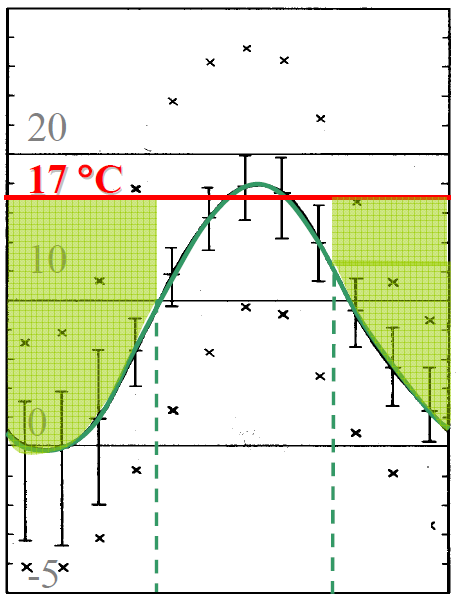
\includegraphics[width=0.55\textwidth]{billeder/graddage.png}
	\caption{Graddagene er illustreret som forskellen mellem basistemperaturen og udetemperaturen (i opvarmningssæsonen angivet med stiplede linjer) og er markeret med grønt.}
	\label{fig:gdmetode}
\end{figure}

Antallet af graddage årligt i Danmark er ca. 3.000. Når bygningsdelenes termiske egenskaber kendes, kan det forventede årlige energiforbrug, $E$, beregnes med ligning \eqref{eq:GD}. De anvendte forudsætninger kan findes i beskrivelsen af casehuset i appendiks \ref{sec:casehus}.

\begin{align}		
E = B_u \m 24 \m G			
\label{eq:GD} 
\end{align}

% \m er i preamble kodet til at gælde som \cdot (gangeprik) for at lette arbejdet

Hvor:
\begin{table}[H]
\begin{tabular}{l|l}
	$E$					& Det forventede energiforbrug [\si{Wh/\text{å}r}] \\
	$B_u$ 				& Bygningens specifikke varmetab ved transmission og ventilation [\si{W/K}] \\
	$24$ 				& Døgnets timer [\si{h/d\text{ø}gn}] \\
	$G$					& Graddage [\si{K d\text{ø}gn/\text{å}r}]
\end{tabular}
\end{table}

Bygningens specifikke varmetab består af bidrag fra transmissionstab og ventilationstab.\fxnote{Skriv færdigt i morgen}


\chapter{Stålmateriale}

Inden der kan regnes på en stålkonstruktion, der skal opsættes i forbindelse med en gennemgribende renovering, beskrives stålet som materiale.

\section{Fremstilling}

\section{Egenskaber}

\fxnote{Husk at skrive om egenskaber ved brand, Jens!}

\subsection{Arbejdskurve}

Den nederste del af ståls arbejdskurve følger principperne om Hook's lov \citep[ s. 419]{fysikbog}.

%% Afrunding %%

\section{Konklusion}
husk at problemformuleringenspunkter skal kunne afkrydses her nede


%%%% Kilder %%%%

\begingroup
	\raggedright
	\bibliography{bibtex/litteratur}							% Litteraturlisten inkluderes
\endgroup


%%%% Fixme-listen %%%%

\newpage														% Ny side til Fixme-listen
\listoffixmes													% Fixme-listen - fjernes til sidst i projektet med "%"


%%%% Appendiks %%%%

\appendix														% Appendiks/bilag start - giver chapter bogstaver i stedet for tal
\clearforchapter												% Sikrer at pagestylen aktiveres paa den rigtige side
\phantomsection													% Kunstigt afsnit, som hyperlinks kan 'holde fast i'
\pdfbookmark[0]{Appendiks}{appendiks}							% Tildeler en klikbar bookmark til den endelige PDF

%% Indstillinger for appendiks (deaktiveret med "%") %%

%\pagestyle{empty}												% Sidehoved/-fod for standardsider aendres til tom for appendiks
%\aliaspagestyle{chapter}{empty}								% Sidehoved/-fod for kapitelsider aendres til tom for appendiks
%\settocdepth{chapter}											% Kun kapitel-niveau vises i ToC
%\addtocontents{toc}{\protect\cftpagenumbersoff{chapter}}		% Sidetal for kapitler fjernes i ToC

%% Filer til appendiks %%

\chapter{Casehus} \label{sec:casehus}


%%%% Bilag %%%%

%\phantomsection												% Kunstigt afsnit, som hyperlinks kan 'holde fast i'
%\addcontentsline{toc}{chapter}{Bilag A \ Navn} 				% Manuelle indgange i indholdsfortegnelsen (naar \includepdf bruges)

%\includepdf[pages={x-y}]{filnavn}								% Inkluder eksterne bilag med \includepdf[pages={x-y}]{filnavn}


\end{document}													% Slutter dokumentet - obligatorisk


